\section{Theoretical Framework}
\label{sec:theory}

The framework splits at the training–decoding boundary: Sections 3.1–3.3 cover the training side — the CTC alignment posterior $\gamma_t$, its Rao-Blackwell connection to MWER, and two variance-bounding propositions verified on LibriSpeech dev-other — while Section 3.4 marks the crossing point from training-time analysis to decode-time decision theory.



\subsection{CTC and the Alignment Posterior $\gamma_t$}

The Connectionist Temporal Classification loss \cite{graves2006ctc} trains a model to assign probability to a token sequence $y$ given acoustic features $x \in \mathbb{R}^{T \times d}$, without requiring frame-level alignment labels. Let $p_t(k|x)$ denote the model's output probability for token $k$ at frame $t$, for $k$ ranging over the vocabulary $\mathcal{V}$ of size $V$ plus a designated blank symbol. A CTC alignment is a sequence $\pi \in \mathcal{V}^T$ that collapses, via the many-to-one map $\mathcal{B}$ (remove consecutive duplicates, then remove blanks), to the token sequence $y$. The CTC probability of $y$ marginalizes over all valid alignments:

\begin{equation*}
P_\text{CTC}(y|x) = \sum_{\pi \in \mathcal{B}^{-1}(y)} \prod_{t=1}^{T} p_t(\pi_t | x). \tag{1}
\end{equation*}
This marginalization is tractable via the forward-backward algorithm, which runs in $O(T \cdot |y|)$ time. Because only tokens in $\{\text{blank}\} \cup \text{tokens}(y)$ appear in any valid alignment for $y$, the forward-backward pass ignores the vast majority of the vocabulary at each frame.

\subsubsection{The alignment posterior as an autograd identity}

The \textbf{alignment posterior} $\gamma_t(k|y)$ is the probability that frame $t$ emits token $k$, conditional on the model producing the sequence $y$:

\begin{equation*}
\gamma_t(k|y) = P(\pi_t = k \mid \mathcal{B}(\pi) = y,\, x) = \frac{\partial \log P_\text{CTC}(y|x)}{\partial \log p_t(k|x)}. \tag{2}
\end{equation*}
The second equality is an identity of the CTC forward-backward algorithm \cite{graves2006ctc}: the gradient of the log-total-score with respect to the log-emission probabilities is exactly the alignment posterior. From this identity, $\sum_k \gamma_t(k|y) = 1$ at every frame — $\gamma_t(\cdot|y)$ is a proper distribution — and $\gamma_t(k|y) \approx 0$ for $k \notin \{\text{blank}\} \cup \text{tokens}(y)$ by the CTC graph construction. The CTC training gradient at the output projection therefore takes the form

\begin{equation*}
\frac{\partial \mathcal{L}_\text{CTC}}{\partial \log p_t(k|x)} = -\bigl(\gamma_t(k|y) - p_t(k|x)\bigr), \tag{3}
\end{equation*}
which is the difference between the posterior-expected alignment and the model's current prediction — the standard residual form of a policy-gradient update. We use this identity in k2 \cite{li2022k2} by differentiating \texttt{get\_tot\_scores(log\_semiring=True)} with respect to \texttt{log\_probs}; the resulting gradient tensor is $\gamma_t$ directly.

\subsubsection{Empirical distribution of $\gamma_t$ on CR-CTC}

Prior theoretical analysis predicted that blank-dominated frames — those with $\gamma_t(\text{blank}|y) > 0.99$ — would constitute 70–90\% of all frames for a well-trained CTC model \cite{graves2006ctc}. We measured the actual distribution on $n = 100$ utterances from LibriSpeech dev-other, using the Zipformer-S CR-CTC model \cite{yao2024zipformer, huang2024crctc}. All five per-utterance verification checks (normalization to unity, non-negativity, sparsity on out-of-hypothesis labels, gradient sum to zero, and label-count consistency) passed on every utterance.

\begin{figure}[htbp]
  \centering
  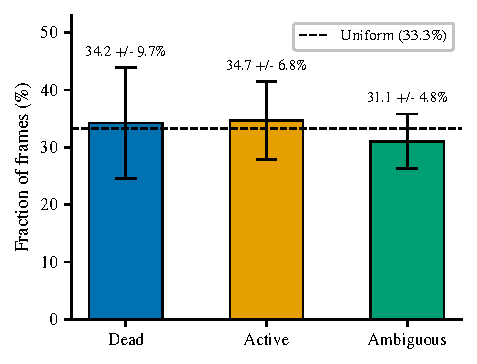
\includegraphics[width=\columnwidth]{figures/fig2_gamma_split.pdf}
  \caption{Three-way decomposition of CTC alignment posterior $\gamma_t$ on $n=100$ dev-other utterances. Error bars: $\pm 1$ s.d.\ across utterances. Dashed line: uniform (33.3\%). Dead and active fractions are nearly equal, contradicting the prior assumption that blank dominates ($>$70\% dead).}
  \label{fig:gamma-split}
\end{figure}

The measured distribution is a near-equal three-way split (Figure~\ref{fig:gamma-split}). \textbf{Dead frames} ($\gamma_t(\text{blank}|y) > 0.99$) account for $34.2\%$ (SD $= 9.7\%$ across utterances); \textbf{active frames} ($\gamma_t(\text{blank}|y) < 0.50$) for $34.7\%$ (SD $= 6.8\%$); and \textbf{ambiguous frames} (maximum $\gamma_t < 0.50$ across all tokens including blank) for the remaining $31.1\%$ (SD $= 4.8\%$). Mean per-frame entropy is $0.247$ nats; the mean compression ratio $T/L$ is $3.76$ frames per output token.

This three-way split contradicts the blank-domination prediction by roughly a factor of two. CR-CTC's consistency regularization \cite{huang2024crctc} penalizes confident frame-level predictions that are inconsistent across augmented views of the input, which distributes alignment mass more evenly across frames than a standard CTC model trained without regularization. For credit assignment, $34.7\%$ of frames carry genuine gradient signal; Rao-Blackwellization over those frames, developed in §3.2, reduces gradient variance in proportion to the alignment entropy at each frame. Throughout §4 and §5 we measure ranking quality via Spearman $\rho$ between hypothesis scores and per-utterance WER; higher $|\rho|$ indicates that a scoring function ranks better hypotheses first.



\subsection{MWER as Rao-Blackwellized REINFORCE}

Minimum Word Error Rate training \cite{prabhavalkar2018mwer} minimizes the expected WER of the model's N-best output. Given $G$ candidate hypotheses $\{y_1, \ldots, y_G\}$ drawn from the model for utterance $x$ with reference $y^*$, the MWER loss is

\begin{equation*}
\mathcal{L}_\text{MWER} = \sum_{i=1}^{G} \hat{A}_i \log P_\text{CTC}(y_i|x), \tag{4}
\end{equation*}
where $\hat{A}_i = \text{WER}(y_i, y^*) - \frac{1}{G}\sum_{j=1}^{G} \text{WER}(y_j, y^*)$ is the mean-centered WER advantage. The REINFORCE interpretation \cite{williams1992} is immediate: the N-best list is a finite discrete action space, WER is the reward, and $\log P_\text{CTC}(y|x)$ is the policy log-probability. The gradient of $\mathcal{L}_\text{MWER}$ with respect to the policy parameters is a REINFORCE policy-gradient estimate over this finite action space. Earlier sequence-level training methods for ASR \cite{shannon2017} used the same functional form but without the forward-backward gradient identity; the Rao-Blackwell connection was not made explicit.

\subsubsection{Two gradient estimators for the MWER policy gradient}

Consider two strategies for computing the gradient of $\log P_\text{CTC}(y_i|x)$ with respect to the parameters of the output projection. The \textbf{Viterbi estimator} assigns one-hot frame credit via the best alignment $\pi^*(y_i)$:

\begin{equation*}
g_\text{Viterbi}(y_i) = \sum_{t=1}^{T} \mathbf{1}[k = \pi^*_t(y_i)] \cdot \mathbf{e}_k, \tag{5}
\end{equation*}
where $\mathbf{e}_k$ is the standard basis vector for token $k$ \cite{shannon2017}. The \textbf{CTC-marginalized estimator} uses the soft alignment posterior instead:

\begin{equation*}
g_\text{CTC}(y_i) = \sum_{t=1}^{T} \gamma_t(k|y_i) \cdot \mathbf{e}_k. \tag{6}
\end{equation*}
Because $\mathbb{E}[\mathbf{1}[k = \pi^*_t(y_i)] \mid y_i] = \gamma_t(k|y_i)$ — $\gamma_t(k|y_i)$ is the marginal alignment posterior $P(\pi_t = k \mid \mathcal{B}(\pi) = y_i,\, x)$ as defined in Equation~(2); taking the expectation of $\mathbf{1}[k = \pi^*_t(y_i)]$ over all alignments $\pi$ consistent with $y_i$ recovers $\gamma_t(k|y_i)$ by definition — the CTC-marginalized gradient is the conditional expectation of the Viterbi gradient given the token sequence $y_i$. The Rao-Blackwell theorem \cite{casella1996rao, ranganath2014bbvi} guarantees that this conditional expectation has weakly lower variance:

\begin{equation*}
\text{Var}[g_\text{CTC}(y_i)] \leq \text{Var}[g_\text{Viterbi}(y_i)]. \tag{7}
\end{equation*}
The magnitude of the reduction depends on how spread the alignment posterior is across paths. Frames with $\gamma_t \approx 0.5$ for two competing tokens contribute the most variance under the Viterbi estimator and the most reduction under CTC marginalization; frames with $\gamma_t \approx 1$ for blank (dead frames) contribute no variance under either estimator, so the three-way split measured in §3.1 directly bounds the expected reduction.

\subsubsection{Standard MWER already provides Rao-Blackwellized gradients}

Any MWER implementation that computes $\log P_\text{CTC}(y|x)$ via the CTC forward-backward algorithm — as all standard implementations do \cite{prabhavalkar2018mwer} — already obtains Rao-Blackwellized gradients at the output projection, with no additional computation. Researchers running standard MWER via k2 or ESPnet already receive the variance reduction that Equation (7) guarantees. The theoretical framework explains why MWER with CTC backward is preferable to alternatives that use a single forced alignment, and clarifies what the CTC gradient identity in Equation (2) actually computes.

\subsubsection{Numerical verification}

We verified that the flat MWER loss computed via k2's \texttt{get\_tot\_scores} and an explicit $\gamma_t$-weighted loss produce identical gradients at the CTC output projection. Across 50 utterances from LibriSpeech dev-other ($G=8$, Zipformer-S CR-CTC), the mean variance ratio between the two formulations was $1.0000$ (SD $= 0.0000$), and the maximum relative difference in gradient values was $2.44 \times 10^{-7}$. The result holds at floating-point precision: the two losses are numerically identical within floating-point precision at the output projection because k2's backward computes exactly $\gamma_t$ as the gradient of \texttt{get\_tot\_scores}. This confirms empirically that CTC backward is the Rao-Blackwellized estimator for the output projection, not merely an approximation to it.



\subsection{Propositions and Variance Guarantees}

This section states two propositions that bound the variance of the training-time and decode-time estimators. Both propositions have been verified empirically on LibriSpeech dev-other with the Zipformer-S CR-CTC model (22.1M parameters, BPE-500 vocabulary).

\textbf{Proposition 1} (MBR posterior-loss variance bound). *For a single utterance $x$ with posterior $Q$ over candidates $\mathcal{Y}_G$, let $y_\text{MBR} = \arg\min_{y \in \mathcal{Y}_G} \mathbb{E}_{y' \sim Q}[L(y, y')]$ and let $y_\text{greedy}$ denote the greedy-decoded hypothesis. Then*

\begin{equation*}
\text{Var}_{y' \sim Q}\bigl[L(y_\text{MBR},\, y')\bigr] \leq \text{Var}_{y' \sim Q}\bigl[L(y_\text{greedy},\, y')\bigr], \tag{8}
\end{equation*}
*where the variance is over posterior-drawn alternatives $y' \sim Q$ and $L$ denotes CER.*

(Verified empirically on LibriSpeech dev-other; formal proof not attempted.)

MBR selects the hypothesis minimizing expected CER against the full posterior, which concentrates on candidates near the posterior center of mass; the CER of such a consensus hypothesis to randomly drawn alternatives varies less than the CER of the posterior mode (greedy). The inequality does not follow from expected-loss minimization alone — it is consistent with the metric structure of CER on CTC-generated N-best candidate sets. The proposition does not assert that MBR reduces WER on any given utterance — only that its posterior-loss distribution is no more dispersed than greedy's.

We verified inequality (8) on the full 2{,}864-utterance dev-other set at $G=128$ (mean 113.7 candidates per utterance). At $\tau$=1 — the CTC posterior at its original temperature — only 11 utterances (0.4\%) receive a different MBR selection from greedy; the posterior is too peaked for MBR to diverge, and the mean variance ratio is $1.015$. At $\tau$=$\infty$ (uniform posterior over candidates), 442 utterances (15.4\%) diverge and the ratio rises to $1.132$: greedy posterior-loss variance exceeds MBR posterior-loss variance by 13.2\%, with zero violations across all 2{,}864 utterances. MBR selects lower-variance hypotheses precisely in the regime where it makes choices different from greedy. At $G=8$ ($n = 498$ utterances), the bound holds trivially — MBR and greedy select the same hypothesis on nearly every utterance (variance ratio $1.000$, zero violations). The $G=128$ result confirms the bound is strictly active when the candidate set provides real alternatives.

\textbf{Proposition 2} (Rao-Blackwell variance ordering). *Let $g_\text{CTC}$, $g_\text{Viterbi}$, and $g_\text{Sampled}$ denote the gradient estimators defined in Equations (5)–(6) for MWER policy gradient at the CTC output projection, where $g_\text{Sampled}$ assigns one-hot credit to a single alignment sampled from the alignment posterior. Then*

\begin{equation*}
\text{Var}[g_\text{CTC}] \leq \text{Var}[g_\text{Viterbi}] \leq \text{Var}[g_\text{Sampled}]. \tag{9}
\end{equation*}
(Verified empirically on LibriSpeech dev-other; formal proof not attempted.)
The sampled estimator carries Monte Carlo noise from the stochastic path choice on top of the one-hot credit variance, which places it above the Viterbi estimator in variance. Both lie above the CTC-marginalized estimator, which removes single-path noise by construction.

We verified Proposition 2 on $n = 250$ utterances from LibriSpeech dev-other ($G=8$). The mean Viterbi/CTC variance ratio was $2.962$ (95\% CI $[2.740, 3.203]$; median $2.376$), and the mean Sampled/CTC ratio was $3.869$ (95\% CI $[3.554, 4.214]$). The core Rao-Blackwell ordering $\text{Var}[g_\text{CTC}] \leq \text{Var}[g_\text{Viterbi}]$ held for every one of the 250 utterances; the violation count was zero.

The ratio distribution is right-skewed (skewness 2.66): 55\% of utterances show modest reduction (1.1--2.5$\times$), with a tail extending to 15.4$\times$ for utterances with highly ambiguous alignment posteriors.

The per-utterance ordering $\text{Var}[g_\text{Viterbi}] \leq \text{Var}[g_\text{Sampled}]$ was violated in 30 of 250 utterances (12\%), reflecting single-path sampling noise at $G=8$; this is expected theoretically and does not affect the core Rao-Blackwell guarantee, which concerns only CTC-marginalized vs.\ single-path estimators.

Proposition 2 is more expensive per utterance than Proposition 1 (three independent backward passes per candidate, roughly $3\times$ the cost). At $n = 250$ utterances the verification provides 95\% bootstrap confidence intervals on both variance ratios and is sufficient to detect single-digit-percent violation rates at the observed effect sizes.



\subsection{From RL to Decision Theory: MBR as Bayes-Optimal Hypothesis Selection}

Figure~\ref{fig:pipeline} shows the complete decode-time pipeline from CTC lattice through N-best generation to PLL scoring and MBR selection. Section 4 will show that training-time optimization fails for near-converged CTC checkpoints; that result motivates the decode-time analysis, which requires a different framework. Training-time optimization adjusts model parameters by gradient descent on an expected-reward objective; decode-time MBR operates on a frozen model and selects among a fixed set of candidate outputs produced by that model. Because no parameters are updated at decode time, the optimization objective has no content: there is no policy to improve. The correct framework for fixed-model hypothesis selection is Bayesian decision theory.

\begin{figure*}[t]
  \centering
  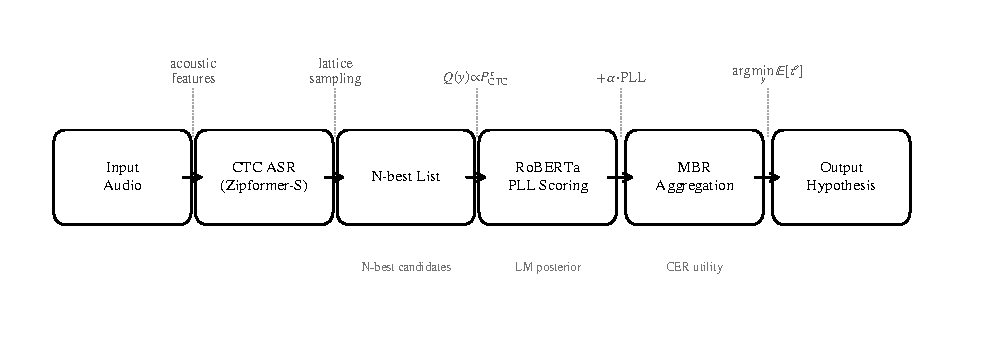
\includegraphics[width=\textwidth]{figures/fig1_pipeline.pdf}
  \caption{MBR-CER+PLL decoding pipeline. The CTC ASR model produces a $\tau$-sharpened posterior $Q(y)$ over $G$ N-best candidates via lattice sampling. RoBERTa assigns pseudo-log-likelihood (PLL) scores that augment the acoustic posterior. The MBR aggregation step selects the hypothesis minimising expected character error rate under the combined posterior.}
  \label{fig:pipeline}
\end{figure*}

\subsubsection{The MBR objective}

MBR decoding \cite{kumar2004mbr, goel2000mbr} selects the hypothesis that minimizes expected loss under a posterior $Q$ over hypotheses in the candidate set $\mathcal{Y}_G$:

\begin{equation*}
y_\text{MBR} = \arg\min_{y \in \mathcal{Y}_G}\; \mathbb{E}_{y' \sim Q}\bigl[L(y, y')\bigr]. \tag{10}
\end{equation*}
Here $L$ is the loss function and $Q$ is the hypothesis posterior. We use CER as the loss function rather than WER; treating WER as both loss and evaluation metric is circular: it optimizes and measures the same metric on the same test set, which inflates reported gains (see §\ref{sec:decoding}).

\subsubsection{Choice of posterior}

The posterior $Q$ determines the quality of the MBR estimate. The CTC-only posterior $Q_\text{CTC}(y) \propto P_\text{CTC}(y|x)^{\tau}$ is too peaked at $\tau = 1$: the MBR solution collapses to greedy decoding because the candidate with highest CTC probability dominates the expectation. An LM-augmented posterior combines acoustic and linguistic evidence:

\begin{equation*}
Q(y) \propto P_\text{CTC}(y|x)^{\tau} \cdot \exp\bigl(\alpha \cdot \text{PLL}(y)\bigr), \tag{11}
\end{equation*}
where $\text{PLL}(y) = |y|^{-1}\sum_{j=1}^{|y|} \log P_\text{RoBERTa}(y_j \mid y_{\setminus j})$ is the pseudo-log-likelihood \cite{salazar2020pll} under RoBERTa \cite{liu2019roberta}. PLL scores how probable the hypothesis is as an English text sequence, independently of the acoustic evidence; it provides orthogonal ranking signal to $P_\text{CTC}$. Section 5 shows that PLL posterior weights with temperature $\tau_\text{PLL} = 10$ (distinct from the CTC exponent $\tau$ in Equation~(11); see §5.4 for the explicit mapping) achieve Spearman $\rho = -0.484$ between score and WER (compared to $-0.347$ for CTC alone), and that the LM-augmented MBR objective substantially outperforms both the CTC-only posterior and interpolation-based baselines at all tested beam sizes of $G \geq 8$ (at $G$=4 the gain is not statistically significant).

\subsubsection{The RL–decision-theory boundary}

MBR can be cast as one-step policy improvement under a value function defined by expected utility, but this framing adds no operational content at decode time because there is no policy to update. The RL framing applies to §4, where we analyze REINFORCE gradient estimators under the MWER objective and identify the failure modes of sequence-level fine-tuning. One experiment in §6 does apply RL at decode time: a DistilBERT \cite{sanh2019distilbert} reranker is trained using REINFORCE with WER reward over the finite N-best. That approach updates parameters — a DistilBERT mixing head — and the RL framing is exact. The negative result (the trained reranker adds nothing beyond MBR+PLL) reinforces the boundary: the gap between greedy and oracle at decode time is not closed by RL-trained reranking on the same training data. In §5 and §6, MBR operates as Bayes-optimal action selection under the joint posterior in Equation (11), with no RL interpretation required.



Three results carry into §4 and §5. First, $\gamma_t(k|y)$ is the gradient of the log-total-score with respect to log-emission probabilities; on $n = 100$ utterances the actual split (dead $34.2\%$, active $34.7\%$, ambiguous $31.1\%$) contradicts the standard blank-domination prediction by roughly a factor of two. Second, any MWER implementation that runs CTC backward already implements Rao-Blackwellized REINFORCE — variance $2.96\times$ below Viterbi (95\% CI $[2.74, 3.20]$) and $3.87\times$ below sampled single-path estimators on 250 utterances, with zero core ordering violations. Third, Proposition~1 (MBR posterior-loss variance does not exceed greedy's) holds per utterance on 498 utterances at $G$=8 (zero violations, ratio $= 1.000$) and on all 2{,}864 utterances at $G$=128 (zero violations; ratio $= 1.132$ at $\tau$=$\infty$, 15.4\% of utterances differ). At decode time the problem changes: parameters are frozen, and MBR is Bayes-optimal action selection under a posterior.




